\documentclass{article}

\usepackage{fancyhdr}
\usepackage{extramarks}
\usepackage{amsmath,mathrsfs,amssymb}
\usepackage{amsthm}
\usepackage{amsfonts}
\usepackage{tikz}
\usepackage[plain]{algorithm}
\usepackage{algpseudocode}
\usepackage[]{mcode}
\usepackage{graphicx}
\usepackage{pgfplots}
\usepackage{xfrac}
\usepackage{caption}
\usepackage{epstopdf}
\usepackage{siunitx}

\usetikzlibrary{automata,positioning}

%
% Basic Document Settings
%

\topmargin=-0.45in
\evensidemargin=0in
\oddsidemargin=0in
\textwidth=6.5in
\textheight=9.0in
\headsep=0.25in

\linespread{1.1}

\pagestyle{fancy}
\lhead{\hmwkAuthorName}
\chead{\hmwkClass\ (\hmwkClassInstructor\ \hmwkClassTime): \hmwkTitle}
\rhead{\firstxmark}
\lfoot{\lastxmark}
\cfoot{\thepage}

\renewcommand\headrulewidth{0.4pt}
\renewcommand\footrulewidth{0.4pt}

\setlength\parindent{0pt}

%
% Create Problem Sections
%

\newcommand{\enterProblemHeader}[1]{
    \nobreak\extramarks{}{Problem \arabic{#1} continued on next page\ldots}\nobreak{}
    \nobreak\extramarks{Problem \arabic{#1} (continued)}{Problem \arabic{#1} continued on next page\ldots}\nobreak{}
}

\newcommand{\exitProblemHeader}[1]{
    \nobreak\extramarks{Problem \arabic{#1} (continued)}{Problem \arabic{#1} continued on next page\ldots}\nobreak{}
    \stepcounter{#1}
    \nobreak\extramarks{Problem \arabic{#1}}{}\nobreak{}
}

\setcounter{secnumdepth}{0}
\newcounter{partCounter}
\newcounter{homeworkProblemCounter}
\setcounter{homeworkProblemCounter}{1}
\nobreak\extramarks{Problem \arabic{homeworkProblemCounter}}{}\nobreak{}

%
% Homework Problem Environment
%
% This environment takes an optional argument. When given, it will adjust the
% problem counter. This is useful for when the problems given for your
% assignment aren't sequential. See the last 3 problems of this template for an
% example.
%
\newenvironment{homeworkProblem}[1][-1]{
    \ifnum#1>0
        \setcounter{homeworkProblemCounter}{#1}
    \fi
    \section{Problem \arabic{homeworkProblemCounter}}
    \setcounter{partCounter}{1}
    \enterProblemHeader{homeworkProblemCounter}
}{
    \exitProblemHeader{homeworkProblemCounter}
}

%
% Homework Details
%   - Title
%   - Due date
%   - Class
%   - Section/Time
%   - Instructor
%   - Author
%

\newcommand{\hmwkTitle}{Tutorial\ 4}
\newcommand{\hmwkDueDate}{May 16, 2016}
\newcommand{\hmwkClass}{Systems Modelling and Control}
\newcommand{\hmwkClassTime}{}
\newcommand{\hmwkClassInstructor}{Damien Hill}
\newcommand{\hmwkAuthorName}{S.Reynolds (262538)}

%
% Title Page
%

\title{
    \vspace{2in}
    \textmd{\textbf{\hmwkClass:\ \hmwkTitle}}\\
    \normalsize\vspace{0.1in}\small{Due\ on\ \hmwkDueDate\ at 3:10pm}\\
    \vspace{0.1in}\large{\textit{\hmwkClassInstructor\ \hmwkClassTime}}
    \vspace{3in}
}

\author{\textbf{\hmwkAuthorName}}
\date{}

\renewcommand{\part}[1]{\textbf{\large Part \Alph{partCounter}}\stepcounter{partCounter}\\}

%
% Various Helper Commands
%

% Useful for algorithms
\newcommand{\alg}[1]{\textsc{\bfseries \footnotesize #1}}

% For derivatives
\newcommand{\deriv}[1]{\frac{\mathrm{d}}{\mathrm{d}x} (#1)}

% For partial derivatives
\newcommand{\pderiv}[2]{\frac{\partial}{\partial #1} (#2)}

% Integral dx
\newcommand{\dx}{\mathrm{d}x}

% Alias for the Solution section header
\newcommand{\solution}{\textbf{\large Solution}}

% Probability commands: Expectation, Variance, Covariance, Bias
\newcommand{\E}{\mathrm{E}}
\newcommand{\Var}{\mathrm{Var}}
\newcommand{\Cov}{\mathrm{Cov}}
\newcommand{\Bias}{\mathrm{Bias}}

\DeclareMathOperator{\sinc}{sinc}

\graphicspath{{./fig/}}

\begin{document}

\maketitle

\pagebreak

%%%%%%%%%%%%%%%%%%%%%%%%%%%%%%%%%%%%%%%%%%%%%%%%%%%%%%%%%%%%%%%%%%%%%%%%%%%%%%%%%%%%%%%%%%%%%%%%%%%%%%%%%%%%%%%%%%%%%%
% Question 1
%%%%%%%%%%%%%%%%%%%%%%%%%%%%%%%%%%%%%%%%%%%%%%%%%%%%%%%%%%%%%%%%%%%%%%%%%%%%%%%%%%%%%%%%%%%%%%%%%%%%%%%%%%%%%%%%%%%%%% 

\begin{homeworkProblem}
    
    
    \textbf{DTFT}\\
    
    \textsc{Question 1}\\
    
    Compute the DTFT of the two discrete time signals shown below. Express the answer in simplest possible form. Plot the amplitude and phase spectra for each signal. The first signals is given by:
    \begin{align*}
	    x[n] = \begin{bmatrix}2 & 2 & 2 & 2 & 2 & -2 & -2 & -2\end{bmatrix}\\
    \end{align*}
    
    Where the first entry of the vector occurs at $n = 0$.
    
    The DTFT is given by:
    \begin{align*}
	    X(\Omega) 	&= \sum_{n = -\infty}^{\infty} x[n] e^{-j \Omega n}\\
				    &= 2(e^{-j \Omega 0} + e^{-j \Omega 1} + e^{-j \Omega 2} + e^{-j \Omega 3} + e^{-j \Omega 4}) - 2(e^{-j \Omega 5}  + e^{-j \Omega 6} + e^{-j \Omega 7})\\
				    &= 2 e^{-2j \Omega} (e^{2j \Omega} + e^{j \Omega} + 1 + e^{-j \Omega} + e^{-2j \Omega}) - 2e^{-6j \Omega}(e^{j \Omega} + 1 + e^{-j \Omega})\\
				    &= 2 e^{-2j \Omega} (2 \cos(2 \Omega) + 2 \cos(\Omega) + 1) - 2e^{-j \Omega}(2\cos(\Omega) + 1)\\
				    &= 4 e^{-2j \Omega} (\cos(2 \Omega) + \cos(\Omega) + \frac{1}{2}) - 4e^{-j \Omega}(\cos(\Omega) + \frac{1}{2})
    \end{align*}
    
    The amplitude and phase plot can be seen in Figure 1.
    
    
    \begin{figure}[H]
    	\centering
    	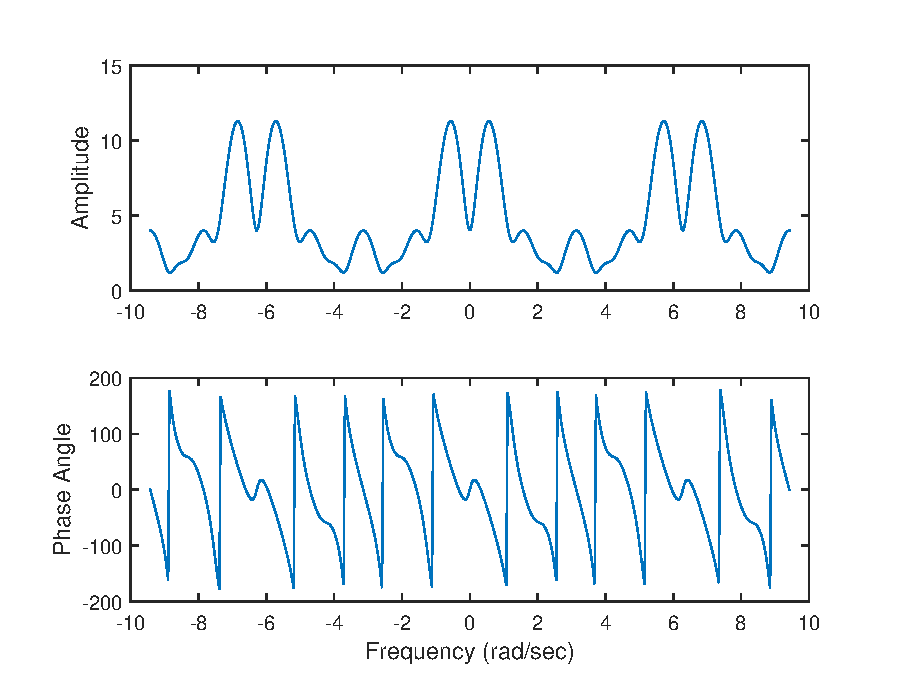
\includegraphics[scale=0.8]{fig1.eps}
    	\captionof{figure}{Bode plot of DTFT of x[n]}
    \end{figure}
    \newpage
    
    The second signal is given by:
    \begin{align*}
    x[n] = [2 \quad 2 \quad 2 \quad 2 \quad 2 \quad 3 \quad 3 \quad 3]\\
    \end{align*}
    
    Where the first entry of the vector occurs at $n = -2$.
    
    The DTFT is given by:
    \begin{align*}
	    X(\Omega) 	&= \sum_{n = -\infty}^{\infty} x[n] e^{-j \Omega n}\\
				    &= 2(e^{2j\Omega} + e^{j\Omega} + 1 + e^{-j\Omega} + e^{-2j\Omega}) + 3(e^{-3j\Omega} + e^{-4j\Omega} + e^{-5j\Omega})\\
				    &= 2(2\cos(2\Omega) + 2\cos(\Omega) + 1) + 3e^{-4j\Omega}(e^{j\Omega} + 1 + e^{-j\Omega})\\
				    &= 4(\cos(2\Omega) + \cos(\Omega) + \frac{1}{2}) + 6e^{-4j\Omega}(\cos(\Omega) + \frac{1}{2})
    \end{align*}
    
    The amplitude and phase plot can be seen in Figure 2.
    
    \begin{figure}[H]
    	\centering
    	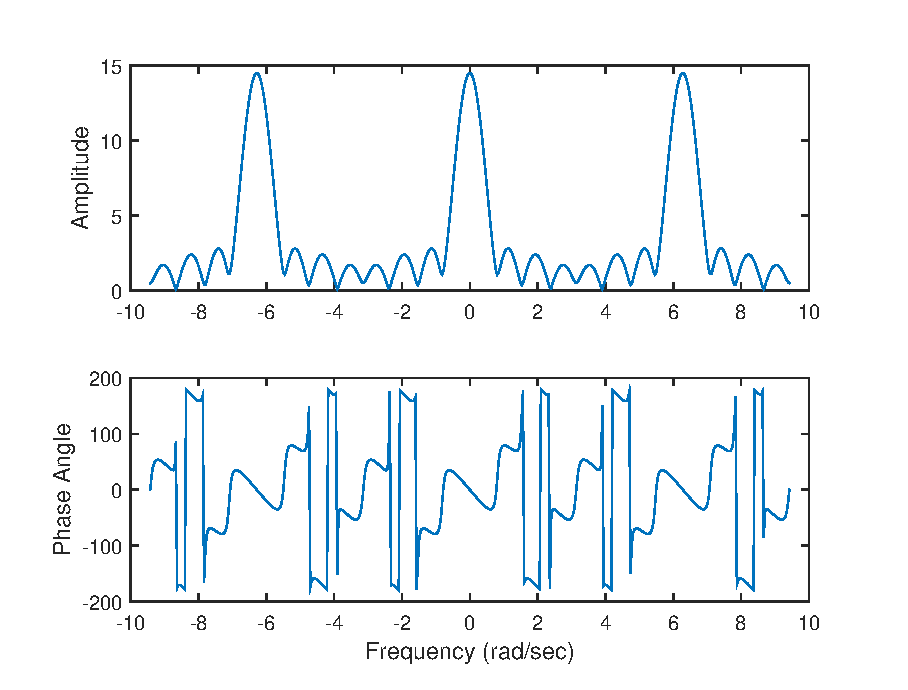
\includegraphics[scale=0.8]{fig2.eps}
    	\captionof{figure}{Bode plot of DTFT of x[n]}
    \end{figure}
\end{homeworkProblem}
\newpage
%%%%%%%%%%%%%%%%%%%%%%%%%%%%%%%%%%%%%%%%%%%%%%%%%%%%%%%%%%%%%%%%%%%%%%%%%%%%%%%%%%%%%%%%%%%%%%%%%%%%%%%%%%%%%%%%%%%%%%
% Question 2
%%%%%%%%%%%%%%%%%%%%%%%%%%%%%%%%%%%%%%%%%%%%%%%%%%%%%%%%%%%%%%%%%%%%%%%%%%%%%%%%%%%%%%%%%%%%%%%%%%%%%%%%%%%%%%%%%%%%%%

\begin{homeworkProblem}
    
    \textbf{DTFT}\\
    
    \textsc{Question 2}\\
    
    A discrete time signals $x[n]$ has a DTFT:
    \begin{align*}
	    X(\Omega) = \frac{1}{e^{j\Omega} + b}
    \end{align*}
    
    \textsc{Question a}\\
    
    If $v[n] = x[n-5]$, then:
    \begin{align*}
	    \mathscr{F} \big\{v[n]\big\} = \frac{e^{-j5\Omega}}{e^{j\Omega} + b}
    \end{align*}
    
    \textsc{Question b}\\
    
    If $v[n] = x[-n]$, then:
    \begin{align*}
	    \mathscr{F} \big\{v[n]\big\} = \frac{1}{e^{-j\Omega} + b}
    \end{align*}
    
    \textsc{Question c}\\
    
    If $v[n] = nx[n]$, then:
    \begin{align*}
	    \mathscr{F}\big\{v[n]\big\} &= j \frac{d}{d\Omega} \bigg(\frac{1}{e^{j\Omega} + b}\bigg)\\
								    &= j (-1) \bigg(\frac{1}{e^{j\Omega} + b}\bigg)^2 j \cdot e^{j\Omega}\\
								    &= \frac{e^{j\Omega}}{(e^{j\Omega} + b)^2}
    \end{align*}
    
    \textsc{Question d}\\
    
    If $v[n] = x[n] - x[n-1]$, then:
    \begin{align*}
	    \mathscr{F}\big\{v[n]\big\} &= \frac{1}{e^{j\Omega} + b} - \frac{1}{e^{-j\Omega} + b}\cdot e^{-j\Omega}\\
								    &= \frac{1}{e^{j\Omega} + b} - \frac{e^{-j\Omega}}{e^{-j\Omega} + b}
    \end{align*}
    
    \textsc{Question e}\\
    
    If $v[n] = x[n]*x[n]$, then:
    \begin{align*}
	    \mathscr{F}\big\{v[n]\big\} &= \mathscr{F}\big\{x[n]\big\} \cdot \mathscr{F}\big\{x[n]\big\}\\
									&= \frac{1}{(e^{j\Omega} + b)^2}
    \end{align*}
    
    \newpage
    
    \textsc{Question f}\\
    
    If $v[n] = x[n]\cos(3n)$, then:
    \begin{align*}
	    \mathscr{F}\big\{v[n]\big\} &= \frac{1}{2} \cdot \bigg( X(\Omega - 3) + X(\Omega + 3) \bigg)\\
								    &= \frac{1}{2} \cdot \bigg( \frac{1}{e^{\Omega - 3} + b} + \frac{1}{e^{\Omega + 3} + b} \bigg)
    \end{align*}
    
	
	\textsc{Question g}\\
	
	If $v[n] = (x[n])^2$, then:
	\begin{align*}
		\mathscr{F}\big\{v[n]\big\} &= X(\Omega) * X(\Omega)\\
									&= \bigg(\frac{1}{e^{j \Omega} + b}\bigg) * \bigg(\frac{1}{e^{j \Omega} + b}\bigg)
	\end{align*}
	
	
	\textsc{Question h}\\
	
	If $v[n] = x[n]e^{j2n}$, then:
	\begin{align*}
		\mathscr{F}\big\{v[n]\big\} &= X(\Omega - 2)\\
									&= \frac{1}{e^{\Omega - 2} + b}
	\end{align*}
\end{homeworkProblem}



%%%%%%%%%%%%%%%%%%%%%%%%%%%%%%%%%%%%%%%%%%%%%%%%%%%%%%%%%%%%%%%%%%%%%%%%%%%%%%%%%%%%%%%%%%%%%%%%%%%%%%%%%%%%%%%%%%%%%%
% Question 3
%%%%%%%%%%%%%%%%%%%%%%%%%%%%%%%%%%%%%%%%%%%%%%%%%%%%%%%%%%%%%%%%%%%%%%%%%%%%%%%%%%%%%%%%%%%%%%%%%%%%%%%%%%%%%%%%%%%%%%

\begin{homeworkProblem}
    
    \textbf{DFT}\\
     
    \textsc{Question 3}\\
	
	Compute the rectangular form of the four point DFT of the following signals, all of which are zero for $n < 0$ and $n \leq 4$. Compare the results with the DFT computed using the MATLAB m-file dft.\\
	
	The Matlab file, dft, is shown below:
	\begin{lstlisting}
		% Discrete Fourier Transform
		
		function Xk = dft(x)
		
			[N,M] = size(x);
		
			if M ~= 1
				x = x';
				N = M;
			end
		
			Xk = zeros(N,1);
			n = 0:(N-1);
		
			for k = 0:(N-1)
				Xk(k+1) = exp(-1i*2*pi*k*n/N)*x;
			end
		end
	\end{lstlisting}
	
	\textsc{Question a}\\
	
	$x[0] = 1$, $x[1] = 0$, $x[2] = 1$, $x[3] = 0$\\
	
	The DFT is given by:
	\begin{align*}
		X_k &= \sum_{n = 0}^{N-1} x[n] e^{-j 2 \pi kn / N}\\
			&= 1 + 1 \cdot e^{-j 2 \pi k 2/4}\\
			&= 1 + e^{-jk\pi}
	\end{align*}
	
	Both the dft algorithm and the analytical solution produce the following results for $k = 0,1,2,3$:
	\begin{verbatim}
		2.0000 + 0.0000i
		0.0000 + 0.0000i
		2.0000 - 0.0000i
		0.0000 + 0.0000i
	\end{verbatim}
	
	\vspace{1cm}
	
	\textsc{Question b}\\
	
	$x[0] = 1$, $x[1] = 0$, $x[2] = -1$, $x[3] = 0$\\
	
	The DFT is given by:
	\begin{align*}
		X_k &= \sum_{n = 0}^{N-1} x[n] e^{-j 2 \pi kn / N}\\
			&= 1 - e^{-jk\pi}
	\end{align*}
	
	Both the dft algorithm and the analytical solution produce the following results for $k = 0,1,2,3$:
	\begin{verbatim}
		0.0000 + 0.0000i
		2.0000 + 0.0000i
		0.0000 - 0.0000i
		2.0000 + 0.0000i
	\end{verbatim}
	
	\newpage
	
	\textsc{Question c}\\
	
	$x[0] = 1$, $x[1] = 1$, $x[2] = -1$, $x[3] = -1$\\
	
	The DFT is given by:
	\begin{align*}
	X_k &= \sum_{n = 0}^{N-1} x[n] e^{-j 2 \pi kn / N}\\
		&= 1 + e^{-j 2 \pi k 1/4} - e^{-jk \pi} - e^{-jk 2 \pi 3/4}\\
		&= 1 + e^{-j k \frac{\pi}{2}} - e^{-jk \pi} - e^{-jk \frac{3\pi}{2}}
	\end{align*}
	
	Both the dft algorithm and the analytical solution produce the following results for $k = 0,1,2,3$:
	\begin{verbatim}
		0.0000 + 0.0000i
		2.0000 - 2.0000i
		0.0000 + 0.0000i
		2.0000 + 2.0000i
	\end{verbatim}
	
	\vspace{1cm}
	
	\textsc{Question d}\\
	
	$x[0] = -1$, $x[1] = 1$, $x[2] = 1$, $x[3] = 1$\\
	
	The DFT is given by:
	\begin{align*}
	X_k &= \sum_{n = 0}^{N-1} x[n] e^{-j 2 \pi kn / N}\\
		&= -1 + e^{-j k \frac{\pi}{2}} - e^{-jk \pi} - e^{-jk \frac{3\pi}{2}}
	\end{align*}
	
	Both the dft algorithm and the analytical solution produce the following results for $k = 0,1,2,3$:
	\begin{verbatim}
		2.0000 + 0.0000i
		-2.0000 - 0.0000i
		-2.0000 - 0.0000i
		-2.0000 - 0.0000i
	\end{verbatim}
	
\end{homeworkProblem}

\newpage

%%%%%%%%%%%%%%%%%%%%%%%%%%%%%%%%%%%%%%%%%%%%%%%%%%%%%%%%%%%%%%%%%%%%%%%%%%%%%%%%%%%%%%%%%%%%%%%%%%%%%%%%%%%%%%%%%%%%%%
% Question 4
%%%%%%%%%%%%%%%%%%%%%%%%%%%%%%%%%%%%%%%%%%%%%%%%%%%%%%%%%%%%%%%%%%%%%%%%%%%%%%%%%%%%%%%%%%%%%%%%%%%%%%%%%%%%%%%%%%%%%%

\begin{homeworkProblem}
    
  \textbf{System Analysis using the DFT}\\
  
  \textsc{Question 4}\\
  
  A mean filter is given by the input/output difference equation:
  \begin{align*}
	  y[n] = \frac{1}{N} \sum_{i=0}^{N-1}x[n-i]
  \end{align*}
  
  \textsc{Question a}\\
  
  Determine the unit-pulse response of the filter.\\
  
  Very simply, the unit-pulse response, $h[n]$, is given by inputting the unit-pulse, $\delta[n]$, to the system:
  \begin{align*}
	  h[n] = \frac{1}{N}\sum_{i=0}^{N-1}\delta[n-i]
  \end{align*} 
  
  \textsc{Question b}\\
  
  Show that the frequency response function, $H(\Omega)$, can be expressed in the form:
  
	  \[ H(\Omega) = \left\{ 
	  \begin{array}{l l}
	  1 & \quad \Omega = 0\\
	  \frac{1 - \cos(N\Omega) + j\sin(N\Omega)}{N(1 - \cos(\Omega) j\sin(\Omega))} & \quad 0 < |\Omega| \leq \pi\\
	  \end{array} \right. \]
  
  The unit impulse response in the frequency domain is given by:
  
  \begin{align*}
	  H(\Omega)		&= \mathscr{F} \big\{h[n]\}\\
					&= \frac{1}{N} \sum_{i = 0}^{N-1} \mathscr{f} \big\{ \delta[n-i]\}\\
					&= \frac{1}{N} \sum_{i = 0}^{N-1} e^{-ji\Omega}\\
					&= \frac{1}{N} \sum_{i = 0}^{N-1} (e^{-j\Omega})^i
  \end{align*}
  
  Now if we define $s$ as:
  \begin{align*}
	  s = \frac{1}{N} \sum_{i = 0}^{N-1} (e^{-j\Omega})^i
  \end{align*}
  
  Hence, $s$ can be written as:
  \begin{align}
	  s = 1 + e^{-j\Omega} + (e^{-j\Omega})^2 + ... + (e^{-j\Omega})^{N-2} + (e^{-j\Omega})^{N-1}
  \end{align}
  
  If we were to multiply both sides of equation (1) by $e^{-j\Omega}$ we get that:
  \begin{align}
	 e^{-j\Omega} s 	&= e^{-j\Omega}\big(1 + e^{-j\Omega} + (e^{-j\Omega})^2 + ... + (e^{-j\Omega})^{N-2} + (e^{-j\Omega})^{N-1}\big) \nonumber \\ 
						&= e^{-j\Omega} + (e^{-j\Omega})^2 + ... + (e^{-j\Omega})^{N-1} + (e^{-j\Omega})^{N}
  \end{align}
  
  If we subtract equation (2) from equation (1), then we get that:
  \begin{align*}
	  s - e^{-j\Omega} s = 1 - (e^{-j\Omega})^{N}
  \end{align*}
  
  Rearranging the above will give us:
  \begin{align*}
	  s = \frac{1 - (e^{-j\Omega})^{N}}{1 - e^{-j\Omega}}
  \end{align*}
  
  Hence, expanding out Euler's formula and simplifying gives us:
  
	  \[ H(\Omega) = \left\{ 
	  \begin{array}{l l}
	  1 & \quad \Omega = 0\\
	  \frac{1 - \cos(N\Omega) + j\sin(N\Omega)}{N(1 - \cos(\Omega) + j\sin(\Omega))} & \quad 0 < |\Omega| \leq \pi\\
	  \end{array} \right. \]
  
  \textsc{Question c \& d}\\
  
  The plots of the magnitude and phase for the transfer functions, when $N=3$ and $N=4$, are shown below in Figures 3 and 4 respectively:
  
  \begin{figure}[H]
  	\centering
  	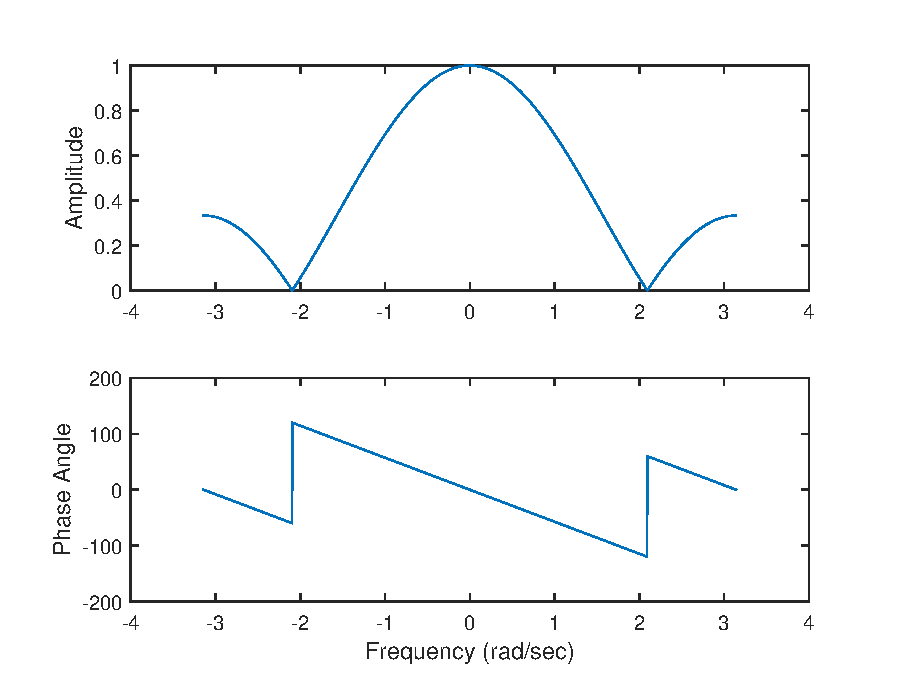
\includegraphics[scale=0.8]{fig3.eps}
  	\captionof{figure}{Bode plot of transfer function with N = 3}
  \end{figure}
  
  \begin{figure}[H]
  	\centering
  	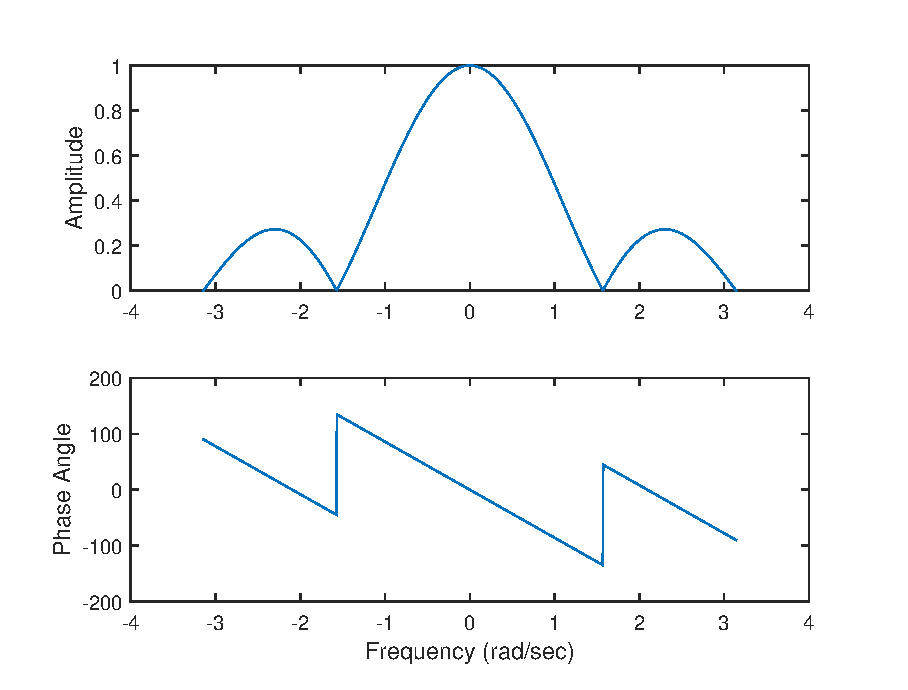
\includegraphics[scale=0.8]{fig4.eps}
  	\captionof{figure}{Bode plot of transfer function with N = 4}
  \end{figure}
  
  \textsc{Question e, part i}\\
  
  Given the signal that $x[n] = 1 \quad \forall \quad n \in \mathbb{Z}$, we can re-write this as $x[n] = \cos(0 \cdot n) \quad \forall \quad n \in\mathbb{Z}$.\\
  
  We note that $\Omega_0 = 0$ and given that $N = 3$, the transfer function, $H(\Omega_0)$, is given by:
  
  \[ H(\Omega_0) = 1 \]
  
  Hence, the input signal, $x[n]$, is a sinusoid, then the solution to the system is given by:
  \begin{align*}
	  y[n]	&= |H(\Omega_0)| \cos(\Omega_0 n + \angle H(\Omega_0))\\
			&= 1 \cdot \cos(0 \cdot n)\\
			&= 1
  \end{align*}
  
  \newpage
  
  The plot of the input and the output can be seen in Figure 5 below.
  %%%%%%%%%%%%%%%%%%%%%%%%%%%
  \begin{figure}[H]
  	\centering
  	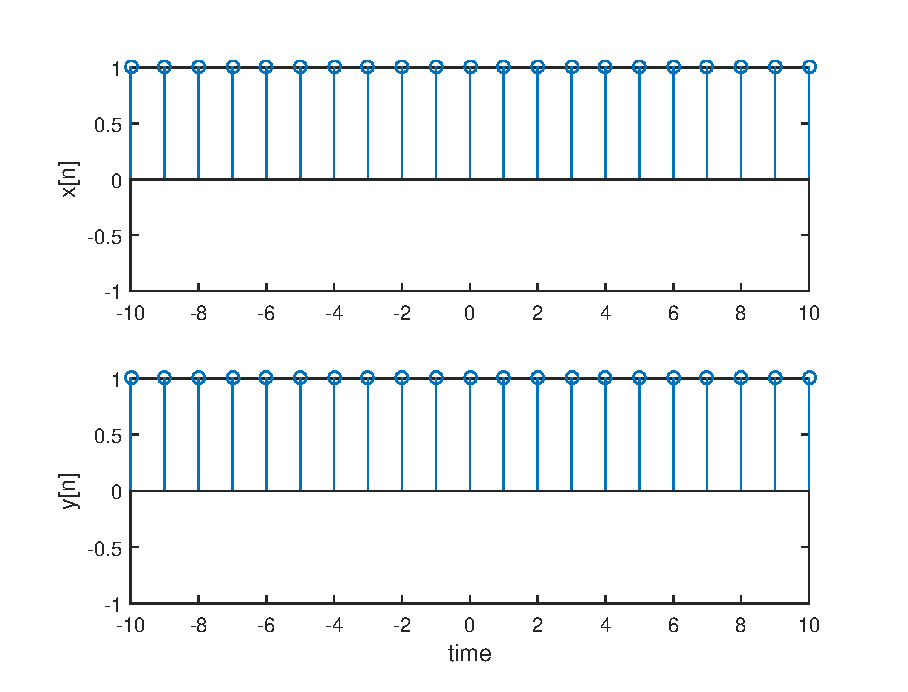
\includegraphics[scale=0.8]{fig5.eps}
  	\captionof{figure}{Time series plot of discete input and output}
  \end{figure}
  %%%%%%%%%%%%%%%%%%%%%%%%%%%
  
  \textsc{Question e, part ii}\\
  
  Given the signal $x[n] = \cos(\frac{\pi}{4} \cdot n) \quad \forall \quad n \in \mathbb{Z}$.\\
  
  We note that $\Omega_0 = \frac{\pi}{4}$ and given that $N = 3$, the transfer function, $H(\Omega_0)$, is given by:
  
  \[ H(\Omega_0) = \frac{1 - \cos(\frac{3 \pi}{4}) + j\sin(\frac{3 \pi}{4})}{3(1 - \cos(\frac{\pi}{4}) + j\sin(\frac{\pi}{4}))} \]
  
  Hence, the input signal, $x[n]$, is a sinusoid, then the solution to the system is given by:
  \begin{align*}
  y[n]	&= |H(\Omega_0)| \cos(\Omega_0 n + \angle H(\Omega_0))\\
  &= 0.8047 \cdot \cos(\frac{\pi}{4} \cdot n -  0.7854)\\
  \end{align*}
  
  \newpage
  
  The plot of the input and the output can be seen in Figure 6 below.
  
  %%%%%%%%%%%%%%%%%%%%%%%%%%%
  \begin{figure}[H]
  	\centering
  	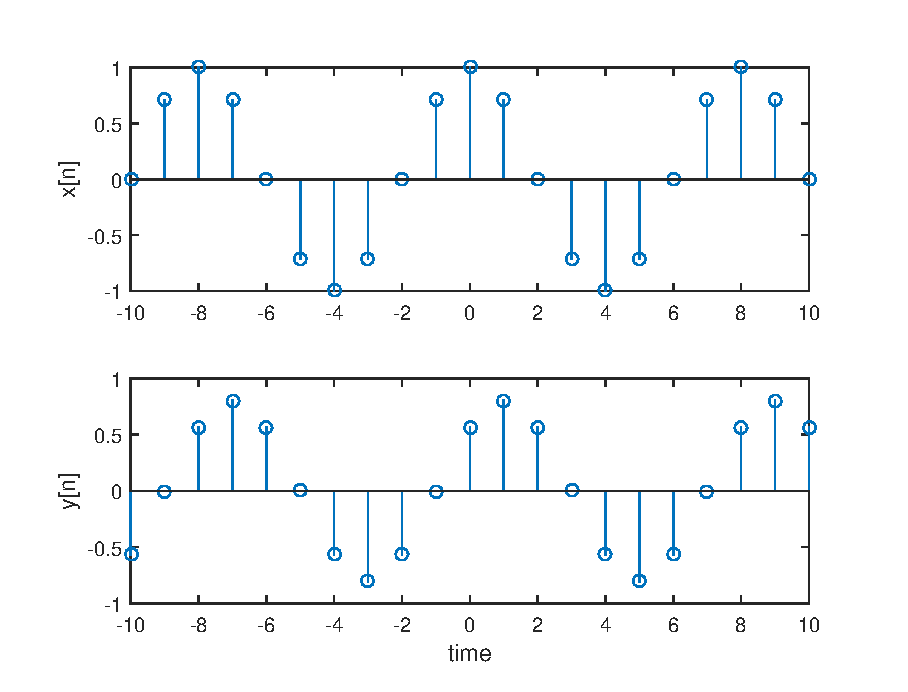
\includegraphics[scale=0.8]{fig6.eps}
  	\captionof{figure}{Time series plot of discete input and output}
  \end{figure}
  %%%%%%%%%%%%%%%%%%%%%%%%%%%
  
  \textsc{Question e, part iii}\\
  
  Given the signal $x[n] = \cos(\frac{\pi}{2} \cdot n) \quad \forall \quad n \in \mathbb{Z}$.\\
  
  We note that $\Omega_0 = \frac{\pi}{2}$ and given that $N = 3$, the transfer function, $H(\Omega_0)$, is given by:
  
  \[ H(\Omega_0) = \frac{1 - \cos(\frac{3 \pi}{2}) + j\sin(\frac{3 \pi}{2})}{3(1 - \cos(\frac{\pi}{2}) + j\sin(\frac{\pi}{2}))} \]
  
  Hence, the input signal, $x[n]$, is a sinusoid, then the solution to the system is given by:
  \begin{align*}
  y[n]	&= |H(\Omega_0)| \cos(\Omega_0 n + \angle H(\Omega_0))\\
  &= 0.3333 \cdot \cos(\frac{\pi}{2} \cdot n - 1.5708)\\
  \end{align*}
  
  \newpage
  
  The plot of the input and the output can be seen in Figure 7 below.
  
  %%%%%%%%%%%%%%%%%%%%%%%%%%%
  \begin{figure}[H]
  	\centering
  	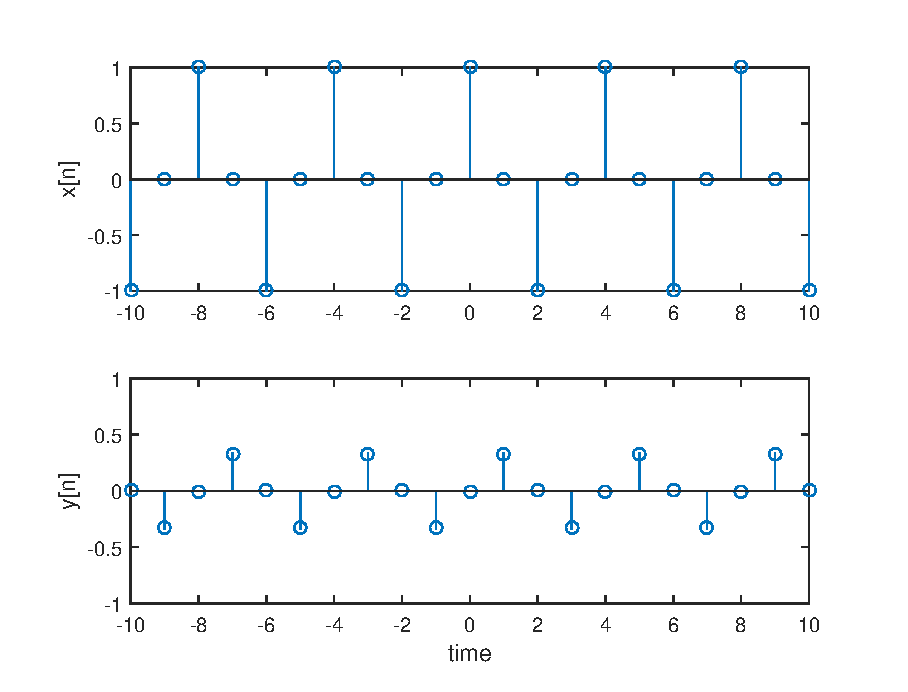
\includegraphics[scale=0.8]{fig7.eps}
  	\captionof{figure}{Time series plot of discete input and output}
  \end{figure}
  %%%%%%%%%%%%%%%%%%%%%%%%%%%
  
  \textsc{Question e, part iv}\\
  
  Given the signal $x[n] = \cos(\frac{\pi}{2} \cdot n) \cdot \sin(\frac{\pi}{4} \cdot n) \quad \forall \quad n \in \mathbb{Z}$.\\
  
  Now, we note a trigonometric identity that states:
  
  \begin{align*}
	  \sin(A) \cdot \cos(B) = \frac{1}{2} \cdot \big(\sin(A + B) +  \sin(A - B)\big)
  \end{align*}
  
  In the case of our problem we see that:
  
  \begin{align*}
	  x[n]	&= \sin(\frac{\pi}{4} \cdot n) \cdot \cos(\frac{\pi}{2} \cdot n)\\
			&= \frac{1}{2} \cdot \big(\sin(\frac{\pi}{4} \cdot n + \frac{\pi}{2} \cdot n) +  \sin(\frac{\pi}{4} \cdot n - \frac{\pi}{2} \cdot n)\big)\\
			&= \frac{1}{2} \cdot \big(\sin(\frac{3\pi}{4} n) +  \sin(-\frac{\pi}{4} n)\big)\\
			&= \frac{1}{2} \cdot \sin(\frac{3\pi}{4} \cdot n) - \frac{1}{2} \cdot \sin(\frac{\pi}{4} \cdot n)\\
			&= \frac{1}{2} \cdot \cos(\frac{3\pi}{4} \cdot n - \frac{\pi}{2}) - \frac{1}{2} \cdot \cos(\frac{\pi}{4} \cdot n - \frac{\pi}{2})
  \end{align*}
  
  Hence, the input signal, $x[n]$, is a sinusoid, then the solution to the system is given by:
  \begin{align*}
	  y[n]	&= |H(\Omega_0)| \cos(\Omega_0 n + \theta +\angle H(\Omega_0))\\
  \end{align*}
  
  If we let $x_1[n] = \frac{1}{2} \cdot \cos(\frac{3\pi}{4} \cdot n - \frac{\pi}{2})$, then $\Omega_0 = \frac{3 \pi}{4}$ and hence:
  \begin{align*}
	  |H\big(\sfrac{3 \pi}{4}\big)| = 0.1381\\
	  \angle H\big(\sfrac{3 \pi}{4}\big) = 0.7854
  \end{align*}
  
  Hence
  \begin{align*}
	  y_1 [n] = \frac{1}{2} \cdot 0.1381 \cdot \cos(\frac{3\pi}{4} - \frac{\pi}{2} \cdot n + 0.7854)
  \end{align*}
  
  If we let $x_2[n] = -\frac{1}{2} \cdot \cos(\frac{\pi}{4} \cdot n - \frac{\pi}{2})$, then $\Omega_0 = \frac{\pi}{4}$ and hence:
  \begin{align*}
  |H\big(\sfrac{3 \pi}{4}\big)| = 0.8047\\
  \angle H\big(\sfrac{3 \pi}{4}\big) = -0.7854
  \end{align*}
  
  Hence
  \begin{align*}
  y_2 [n] = -\frac{1}{2} \cdot 0.8047 \cdot \cos(\frac{\pi}{4} \cdot n - \frac{\pi}{2} - 0.7854)
  \end{align*}
  
  Superposition allows to superimpose two output signals from two input signals, hence:
  \begin{align*}
	  y[n]	= y_1[n] + y_2[n]\\
  \end{align*}
  
  Hence, the output, $y[n]$, for the input, x[n], is give by:
  \begin{align*}
	 y[n] &= \frac{1}{2} \cdot 0.1381 \cdot \cos(\frac{3\pi}{4} - \frac{\pi}{2} \cdot n + 0.7854) - \frac{1}{2} \cdot 0.8047 \cdot \cos(\frac{\pi}{4} \cdot n - \frac{\pi}{2} - 0.7854)
  \end{align*}
  The plot of the input and the output can be seen in Figure 8 below.
  
  %%%%%%%%%%%%%%%%%%%%%%%%%%%
  \begin{figure}[H]
  	\centering
  	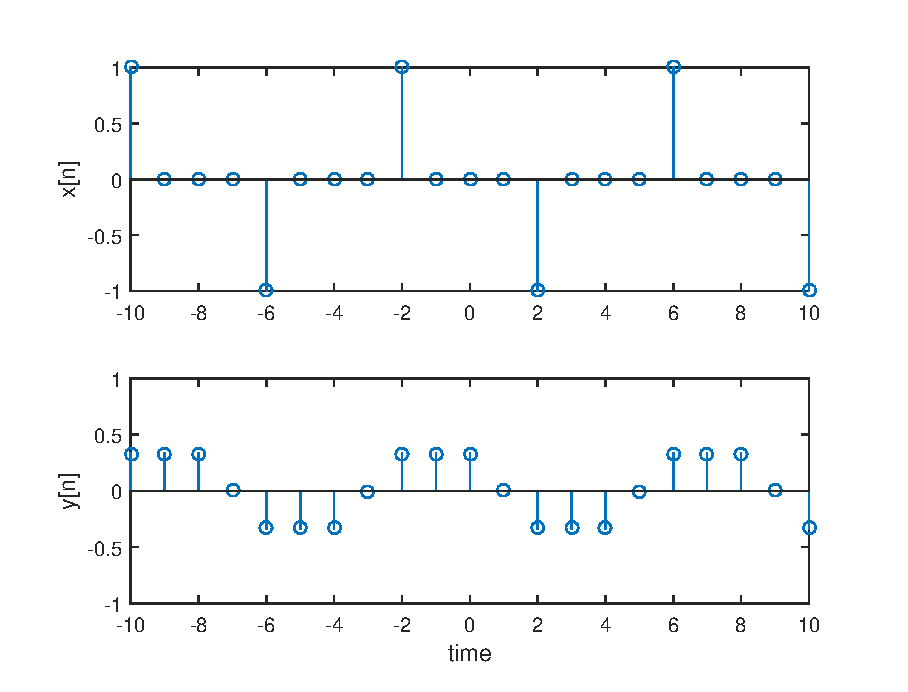
\includegraphics[scale=0.8]{fig8.eps}
  	\captionof{figure}{Time series plot of discete input and output}
  \end{figure}
  %%%%%%%%%%%%%%%%%%%%%%%%%%%
  
\end{homeworkProblem}

\end{document}
